% Secciones 1, 10, 11, 12 y anexos (tarea R3) - autor: Persona C.
% \parte=1 imprime la introduccion; \parte=2 imprime pruebas, conclusiones y anexos.
\ifnum\parte=1

\section{Introducción y dominio seleccionado}

Los lenguajes de programación y los lenguajes de dominio específico (DSL) necesitan mecanismos que verifiquen si
una secuencia de símbolos cumple una estructura formal. Este proyecto diseña e implementa, \emph{desde cero},
un analizador sintáctico para un pequeño DSL, aplicando los contenidos del curso: gramáticas libres de contexto (GLC),
eliminación de recursión por la izquierda, factorización, conjuntos FIRST y FOLLOW, tabla predictiva LL(1),
construcción de árboles sintácticos y detección de errores.

\paragraph{Dominio escogido.} Se eligió la \textbf{automatización de una casa inteligente (IoT)}, el ejemplo
orientativo del enunciado. El usuario describe \emph{reglas} del tipo ``cuando ocurra esta condición, ejecuta estas acciones'':
\begin{center}\texttt{WHEN temperatura > 28 AND humedad < 40 THEN encender ventilador;}\end{center}
Este dominio es adecuado porque (i)~las reglas condición--acción son naturales y fáciles de validar, (ii)~las condiciones admiten
conectores lógicos, negación y agrupación, lo que obliga a resolver precedencia y asociatividad en la gramática, y
(iii)~las acciones admiten parámetros, lo que enriquece la sintaxis sin perder la propiedad LL(1).

\paragraph{Alcance.} El lenguaje se llama \textbf{DomoDSL}. Se entregan: la especificación del lenguaje, la GLC y su
análisis, FIRST/FOLLOW, la tabla LL(1), \textbf{dos} analizadores predictivos (descenso recursivo y dirigido por tabla),
AST y árbol de derivación, mensajes de error localizados, 46 casos de prueba y 18 pruebas unitarias.

\paragraph{Estructura del informe.} Sigue la organización sugerida en el enunciado: especificación del lenguaje
(sección~2), gramática (3), análisis (4), FIRST y FOLLOW (5), tabla LL(1) (6), parser (7), árboles (8), errores (9),
pruebas (10), conclusiones (11) y anexos (12).

\fi
\ifnum\parte=2

\section{Casos de prueba}

Se documentan \textbf{46 casos}: 12 válidas, 20 inválidas y 14 casos límite (el enunciado exige 10, 10 y 5; la rúbrica premia
25 o más pruebas variadas). Cada caso se ejecutó con \textbf{ambos analizadores}; el resultado de las tablas es el obtenido por el programa
(\texttt{python ejecutar\_pruebas.py}). Resultado global: \textbf{46/46 casos correctos}.
Además hay 18 pruebas unitarias (\texttt{python -m unittest}) que verifican el léxico, FIRST, FOLLOW, la ausencia de conflictos, la precedencia
y asociatividad del AST y la posición de los errores. Los casos de entradas muy largas (L05--L07) se muestran abreviados; su texto completo se genera
en \texttt{casos\_prueba.py}.

\begin{landscape}
\subsection{Entradas sintácticamente válidas}
\begin{longtable}{@{}>{\raggedright\arraybackslash}p{0.9cm} >{\raggedright\arraybackslash}p{6.4cm} >{\raggedright\arraybackslash}p{3.2cm} >{\raggedright\arraybackslash}p{6.8cm} >{\raggedright\arraybackslash}p{4.4cm}@{}}
\toprule
\textbf{ID} & \textbf{Entrada} & \textbf{Resultado esperado} & \textbf{Resultado obtenido} & \textbf{Observación} \\
\midrule
\endhead
V01 & \footnotesize \texttt{WHEN temperatura > 28 THEN encender ventilador;} & \footnotesize ACEPTA & \footnotesize ACEPTA \ok & \footnotesize Regla mínima del enunciado \\
\addlinespace[2pt]
V02 & \footnotesize \texttt{WHEN movimiento == TRUE THEN activar alarma;} & \footnotesize ACEPTA & \footnotesize ACEPTA \ok & \footnotesize Valor booleano \\
\addlinespace[2pt]
V03 & \footnotesize \texttt{WHEN temperatura > 28 AND humedad < 40 THEN encender ventilador;} & \footnotesize ACEPTA & \footnotesize ACEPTA \ok & \footnotesize Conector AND \\
\addlinespace[2pt]
V04 & \footnotesize \texttt{WHEN luz < 100 OR hora >= 20 THEN encender lampara;} & \footnotesize ACEPTA & \footnotesize ACEPTA \ok & \footnotesize Conector OR y operador >= \\
\addlinespace[2pt]
V05 & \footnotesize \texttt{WHEN NOT puerta == TRUE THEN activar alarma;} & \footnotesize ACEPTA & \footnotesize ACEPTA \ok & \footnotesize Extensión: NOT \\
\addlinespace[2pt]
V06 & \footnotesize \texttt{WHEN (temperatura > 30 OR humedad > 80) AND presencia == TRUE THEN encender aire;} & \footnotesize ACEPTA & \footnotesize ACEPTA \ok & \footnotesize Extensión: paréntesis (agrupación) \\
\addlinespace[2pt]
V07 & \footnotesize \texttt{WHEN temperatura > 28 THEN encender ventilador 3, activar alarma;} & \footnotesize ACEPTA & \footnotesize ACEPTA \ok & \footnotesize Extensión: múltiples acciones y parámetro \\
\addlinespace[2pt]
V08 & \footnotesize \texttt{WHEN temperatura >= 26.5 THEN ajustar termostato 22 TRUE;} & \footnotesize ACEPTA & \footnotesize ACEPTA \ok & \footnotesize Número decimal y varios parámetros \\
\addlinespace[2pt]
V09 & \footnotesize \texttt{WHEN temperatura > 28 THEN encender ventilador;\textbackslash{}nWHEN movimiento == TRUE THEN activar alarma;} & \footnotesize ACEPTA & \footnotesize ACEPTA \ok & \footnotesize Dos reglas en líneas distintas \\
\addlinespace[2pt]
V10 & \footnotesize \texttt{WHEN a != b THEN x y;} & \footnotesize ACEPTA & \footnotesize ACEPTA \ok & \footnotesize Comparación ID contra ID \\
\addlinespace[2pt]
V11 & \footnotesize \texttt{WHEN NOT NOT a == 1 THEN x y;} & \footnotesize ACEPTA & \footnotesize ACEPTA \ok & \footnotesize NOT anidado \\
\addlinespace[2pt]
V12 & \footnotesize \texttt{WHEN a > 1 AND (b < 2 OR NOT (c == TRUE)) THEN x y 1 2 3 TRUE FALSE z;} & \footnotesize ACEPTA & \footnotesize ACEPTA \ok & \footnotesize Combina NOT, paréntesis y lista larga de parámetros \\
\addlinespace[2pt]
\bottomrule
\end{longtable}
\subsection{Entradas sintácticamente inválidas}
\begin{longtable}{@{}>{\raggedright\arraybackslash}p{0.9cm} >{\raggedright\arraybackslash}p{6.4cm} >{\raggedright\arraybackslash}p{3.2cm} >{\raggedright\arraybackslash}p{6.8cm} >{\raggedright\arraybackslash}p{4.4cm}@{}}
\toprule
\textbf{ID} & \textbf{Entrada} & \textbf{Resultado esperado} & \textbf{Resultado obtenido} & \textbf{Observación} \\
\midrule
\endhead
I01 & \footnotesize \texttt{WHEN temperatura > 28 encender ventilador;} & \footnotesize RECHAZA (el mensaje menciona «la palabra reservada THEN») & \footnotesize RECHAZA \ok\newline \scriptsize Error sintáctico [1:23]: se esperaba la palabra reservada THEN (o un conector AND / OR) después de la condición, pero se encontró el identificador 'encender'. & \footnotesize Falta THEN \\
\addlinespace[2pt]
I02 & \footnotesize \texttt{WHEN temperatura > THEN encender ventilador;} & \footnotesize RECHAZA (el mensaje menciona «después del operador >») & \footnotesize RECHAZA \ok\newline \scriptsize Error sintáctico [1:20]: se esperaba un valor (número, TRUE, FALSE o identificador) después del operador >, pero se encontró la palabra reservada THEN. & \footnotesize Falta el valor tras el operador \\
\addlinespace[2pt]
I03 & \footnotesize \texttt{WHEN temperatura 28 THEN encender ventilador;} & \footnotesize RECHAZA (el mensaje menciona «después de 'temperatura'») & \footnotesize RECHAZA \ok\newline \scriptsize Error sintáctico [1:18]: se esperaba un operador relacional ('>', '<', '>=', '<=', '==', '!=') después de 'temperatura', pero se encontró el número 28. & \footnotesize Falta el operador relacional \\
\addlinespace[2pt]
I04 & \footnotesize \texttt{temperatura > 28 THEN encender ventilador;} & \footnotesize RECHAZA (el mensaje menciona «la palabra reservada WHEN») & \footnotesize RECHAZA \ok\newline \scriptsize Error sintáctico [1:1]: se esperaba la palabra reservada WHEN al inicio de una regla, pero se encontró el identificador 'temperatura'. & \footnotesize La regla no comienza con WHEN \\
\addlinespace[2pt]
I05 & \footnotesize \texttt{WHEN temperatura > 28 THEN encender ventilador} & \footnotesize RECHAZA (el mensaje menciona «';'») & \footnotesize RECHAZA \ok\newline \scriptsize Error sintáctico [1:47]: se esperaba ';' al final de la regla (o ',' para encadenar otra acción), pero se encontró el fin de la entrada. & \footnotesize Falta el punto y coma final \\
\addlinespace[2pt]
I06 & \footnotesize \texttt{WHEN temperatura > 28 THEN ;} & \footnotesize RECHAZA (el mensaje menciona «el nombre de una acción») & \footnotesize RECHAZA \ok\newline \scriptsize Error sintáctico [1:28]: se esperaba el nombre de una acción (identificador) después de THEN, pero se encontró el símbolo ';'. & \footnotesize Regla sin acción \\
\addlinespace[2pt]
I07 & \footnotesize \texttt{WHEN temperatura > 28 THEN encender;} & \footnotesize RECHAZA (el mensaje menciona «después de la acción 'encender'») & \footnotesize RECHAZA \ok\newline \scriptsize Error sintáctico [1:36]: se esperaba el dispositivo u objeto (identificador) después de la acción 'encender', pero se encontró el símbolo ';'. & \footnotesize Acción sin dispositivo \\
\addlinespace[2pt]
I08 & \footnotesize \texttt{WHEN (temperatura > 28 THEN encender ventilador;} & \footnotesize RECHAZA (el mensaje menciona «')' para cerrar el paréntesis») & \footnotesize RECHAZA \ok\newline \scriptsize Error sintáctico [1:24]: se esperaba ')' para cerrar el paréntesis abierto en la columna 6, pero se encontró la palabra reservada THEN. & \footnotesize Paréntesis sin cerrar \\
\addlinespace[2pt]
I09 & \footnotesize \texttt{WHEN temperatura > 28) THEN encender ventilador;} & \footnotesize RECHAZA (el mensaje menciona «sin su '(' correspondiente») & \footnotesize RECHAZA \ok\newline \scriptsize Error sintáctico [1:22]: paréntesis de cierre ')' sin su '(' correspondiente. & \footnotesize Paréntesis de cierre sobrante \\
\addlinespace[2pt]
I10 & \footnotesize \texttt{WHEN temperatura > 28 AND THEN encender ventilador;} & \footnotesize RECHAZA (el mensaje menciona «después de AND») & \footnotesize RECHAZA \ok\newline \scriptsize Error sintáctico [1:27]: se esperaba una condición (un identificador, NOT o '(') después de AND, pero se encontró la palabra reservada THEN. & \footnotesize AND sin segundo operando \\
\addlinespace[2pt]
I11 & \footnotesize \texttt{WHEN temperatura > 28 OR OR humedad < 3 THEN x y;} & \footnotesize RECHAZA (el mensaje menciona «después de OR») & \footnotesize RECHAZA \ok\newline \scriptsize Error sintáctico [1:26]: se esperaba una condición (un identificador, NOT o '(') después de OR, pero se encontró la palabra reservada OR. & \footnotesize Dos OR seguidos \\
\addlinespace[2pt]
I12 & \footnotesize \texttt{WHEN temperatura = 28 THEN encender ventilador;} & \footnotesize RECHAZA (el mensaje menciona «¿quiso escribir '=='») & \footnotesize RECHAZA \ok\newline \scriptsize Error léxico [1:18]: símbolo no reconocido '='. ¿quiso escribir '==' para comparar? & \footnotesize Error léxico: '=' en vez de '==' \\
\addlinespace[2pt]
I13 & \footnotesize \texttt{WHEN temperatura > 28 THEN encender ventilador;\textbackslash{}nWHEN humedad < 40 THEN encender bomba} & \footnotesize RECHAZA (el mensaje menciona «línea 2») & \footnotesize RECHAZA \ok\newline \scriptsize Error sintáctico [2:38]: se esperaba ';' al final de la regla (o ',' para encadenar otra acción), pero se encontró el fin de la entrada. & \footnotesize Segunda regla sin ';' (error localizado en la línea 2) \\
\addlinespace[2pt]
I14 & \footnotesize \texttt{WHEN 28 > temperatura THEN encender ventilador;} & \footnotesize RECHAZA (el mensaje menciona «el número 28») & \footnotesize RECHAZA \ok\newline \scriptsize Error sintáctico [1:6]: se esperaba una condición (un identificador, NOT o '(') después de WHEN, pero se encontró el número 28. & \footnotesize Un número a la izquierda del operador \\
\addlinespace[2pt]
I15 & \footnotesize \texttt{WHEN temperatura > 28 THEN encender ventilador @;} & \footnotesize RECHAZA (el mensaje menciona «símbolo no reconocido '@'») & \footnotesize RECHAZA \ok\newline \scriptsize Error léxico [1:48]: símbolo no reconocido '@'. & \footnotesize Error léxico: carácter no válido \\
\addlinespace[2pt]
I16 & \footnotesize \texttt{WHEN temperatura > 28 THEN encender ventilador;;} & \footnotesize RECHAZA (el mensaje menciona «una nueva regla (WHEN) o el fin de la entrada») & \footnotesize RECHAZA \ok\newline \scriptsize Error sintáctico [1:48]: se esperaba una nueva regla (WHEN) o el fin de la entrada después de ';', pero se encontró el símbolo ';'. & \footnotesize Punto y coma duplicado \\
\addlinespace[2pt]
I17 & \footnotesize \texttt{WHEN temperatura > 28 THEN encender ventilador, ;} & \footnotesize RECHAZA (el mensaje menciona «después de ','») & \footnotesize RECHAZA \ok\newline \scriptsize Error sintáctico [1:49]: se esperaba el nombre de una acción (identificador) después de ',', pero se encontró el símbolo ';'. & \footnotesize Coma sin acción posterior \\
\addlinespace[2pt]
I18 & \footnotesize \texttt{WHEN NOT THEN x y;} & \footnotesize RECHAZA (el mensaje menciona «después de NOT») & \footnotesize RECHAZA \ok\newline \scriptsize Error sintáctico [1:10]: se esperaba una condición (un identificador, NOT o '(') después de NOT, pero se encontró la palabra reservada THEN. & \footnotesize NOT sin operando \\
\addlinespace[2pt]
I19 & \footnotesize \texttt{WHEN a > 1 THEN x y WHEN b < 3 THEN z w;} & \footnotesize RECHAZA (el mensaje menciona «la palabra reservada WHEN») & \footnotesize RECHAZA \ok\newline \scriptsize Error sintáctico [1:21]: se esperaba ';' al final de la regla (o ',' para encadenar otra acción), pero se encontró la palabra reservada WHEN. & \footnotesize Falta ';' entre dos reglas \\
\addlinespace[2pt]
I20 & \footnotesize \texttt{WHEN a > 1 THEN 5 ventilador;} & \footnotesize RECHAZA (el mensaje menciona «el nombre de una acción») & \footnotesize RECHAZA \ok\newline \scriptsize Error sintáctico [1:17]: se esperaba el nombre de una acción (identificador) después de THEN, pero se encontró el número 5. & \footnotesize La acción debe ser un identificador \\
\addlinespace[2pt]
\bottomrule
\end{longtable}
\subsection{Casos límite}
\begin{longtable}{@{}>{\raggedright\arraybackslash}p{0.9cm} >{\raggedright\arraybackslash}p{6.4cm} >{\raggedright\arraybackslash}p{3.2cm} >{\raggedright\arraybackslash}p{6.8cm} >{\raggedright\arraybackslash}p{4.4cm}@{}}
\toprule
\textbf{ID} & \textbf{Entrada} & \textbf{Resultado esperado} & \textbf{Resultado obtenido} & \textbf{Observación} \\
\midrule
\endhead
L01 & \footnotesize \texttt{(cadena vacía)} & \footnotesize RECHAZA (el mensaje menciona «la entrada está vacía») & \footnotesize RECHAZA \ok\newline \scriptsize Error sintáctico [1:1]: la entrada está vacía: se esperaba al menos una regla que comience con la palabra reservada WHEN. & \footnotesize Entrada vacía \\
\addlinespace[2pt]
L02 & \footnotesize \texttt{(espacios, tabulaciones y saltos de línea)} & \footnotesize RECHAZA (el mensaje menciona «la entrada está vacía») & \footnotesize RECHAZA \ok\newline \scriptsize Error sintáctico [3:1]: la entrada está vacía: se esperaba al menos una regla que comience con la palabra reservada WHEN. & \footnotesize Solo espacios y saltos de línea \\
\addlinespace[2pt]
L03 & \footnotesize \texttt{WHEN} & \footnotesize RECHAZA (el mensaje menciona «el fin de la entrada») & \footnotesize RECHAZA \ok\newline \scriptsize Error sintáctico [1:5]: se esperaba una condición (un identificador, NOT o '(') después de WHEN, pero se encontró el fin de la entrada. & \footnotesize Solo la palabra WHEN \\
\addlinespace[2pt]
L04 & \footnotesize \texttt{WHEN a>1 THEN x y;} & \footnotesize ACEPTA & \footnotesize ACEPTA \ok & \footnotesize Regla mínima sin espacios alrededor del operador \\
\addlinespace[2pt]
L05 & \footnotesize \texttt{WHEN ((((((((((((((((((((a > 1)))))))))))))))))))) THEN x y;  [20 niveles]} & \footnotesize ACEPTA & \footnotesize ACEPTA \ok & \footnotesize 20 niveles de paréntesis anidados \\
\addlinespace[2pt]
L06 & \footnotesize \texttt{WHEN s0 > 0 AND s1 > 1 AND ... AND s199 > 199 THEN x y;  [200 comparaciones]} & \footnotesize ACEPTA & \footnotesize ACEPTA \ok & \footnotesize 200 comparaciones unidas por AND \\
\addlinespace[2pt]
L07 & \footnotesize \texttt{WHEN s0 > 0 THEN activar r0;  ...  WHEN s99 > 99 THEN activar r99;  [100 reglas]} & \footnotesize ACEPTA & \footnotesize ACEPTA \ok & \footnotesize Programa con 100 reglas \\
\addlinespace[2pt]
L08 & \footnotesize \texttt{when temperatura > 28 then encender ventilador;} & \footnotesize ACEPTA & \footnotesize ACEPTA \ok & \footnotesize Palabras reservadas en minúsculas (el lexer es insensible a mayúsculas) \\
\addlinespace[2pt]
L09 & \footnotesize \texttt{WHEN sensor\_1 > 0.5 THEN abrir valvula\_2 100;} & \footnotesize ACEPTA & \footnotesize ACEPTA \ok & \footnotesize Identificadores con \_ y dígitos; decimal \\
\addlinespace[2pt]
L10 & \footnotesize \texttt{WHEN when > 1 THEN x y;} & \footnotesize RECHAZA (el mensaje menciona «la palabra reservada WHEN») & \footnotesize RECHAZA \ok\newline \scriptsize Error sintáctico [1:6]: se esperaba una condición (un identificador, NOT o '(') después de WHEN, pero se encontró la palabra reservada WHEN. & \footnotesize Palabra reservada usada como identificador \\
\addlinespace[2pt]
L11 & \footnotesize \texttt{WHEN a > 2abc THEN x y;} & \footnotesize RECHAZA (el mensaje menciona «el identificador 'abc'») & \footnotesize RECHAZA \ok\newline \scriptsize Error sintáctico [1:11]: se esperaba la palabra reservada THEN (o un conector AND / OR) después de la condición, pero se encontró el identificador 'abc'. & \footnotesize Número pegado a letras: se separa en NUM + ID \\
\addlinespace[2pt]
L12 & \footnotesize \texttt{WHEN a > 1\textbackslash{}nTHEN x\textbackslash{}n;} & \footnotesize RECHAZA (el mensaje menciona «línea 3») & \footnotesize RECHAZA \ok\newline \scriptsize Error sintáctico [3:1]: se esperaba el dispositivo u objeto (identificador) después de la acción 'x', pero se encontró el símbolo ';'. & \footnotesize Error en la línea 3 (acción sin dispositivo, con saltos de línea) \\
\addlinespace[2pt]
L13 & \footnotesize \texttt{WHEN a > 1. THEN x y;} & \footnotesize RECHAZA (el mensaje menciona «símbolo no reconocido '.'») & \footnotesize RECHAZA \ok\newline \scriptsize Error léxico [1:11]: símbolo no reconocido '.'. & \footnotesize Decimal incompleto '1.' \\
\addlinespace[2pt]
L14 & \footnotesize \texttt{WHEN ((a > 1)) THEN x y;} & \footnotesize ACEPTA & \footnotesize ACEPTA \ok & \footnotesize Paréntesis redundantes \\
\addlinespace[2pt]
\bottomrule
\end{longtable}
\end{landscape}

\paragraph{Análisis de los casos límite.} Cubren: entrada vacía y solo espacios (L01--L02); regla truncada (L03); regla mínima sin espacios (L04);
anidamiento profundo de 20 paréntesis (L05); 200 conectores (L06) y 100 reglas (L07), que prueban que los ciclos no desbordan la pila;
mayúsculas/minúsculas (L08); identificadores con \texttt{\_} y dígitos y decimales (L09); palabra reservada como identificador (L10);
número pegado a letras (L11); error ubicado en la línea 3 de una entrada multilínea (L12); decimal incompleto (L13) y paréntesis redundantes (L14).

\section{Conclusiones}

\begin{itemize}[nosep]
\item Se diseñó un DSL completo para automatización de una casa inteligente y se formalizó con una GLC de 24 producciones,
obtenida transformando una primera versión natural ($G_0$) que era recursiva por la izquierda, tenía prefijos comunes y era ambigua.
\item Las transformaciones (eliminación de recursión izquierda, factorización y estratificación por precedencia) llevaron a una gramática
\textbf{LL(1) sin conflictos}, comprobada con FIRST, FOLLOW, conjuntos de selección y la tabla.
\item Se implementaron \textbf{dos analizadores predictivos escritos a mano} (descenso recursivo y dirigido por tabla) que coinciden en los 46 casos;
el primero construye un AST legible y el segundo el árbol de derivación y una traza.
\item El manejo de errores entrega mensajes útiles y localizados (línea, columna, posición, puntero), sensibles al contexto.
\item La extensión (\texttt{NOT}, paréntesis, acciones múltiples con parámetros) no es decorativa: modifica la gramática, FIRST/FOLLOW, la tabla, ambos
parsers y las pruebas.
\end{itemize}

\paragraph{Limitaciones y trabajo futuro.} Un solo error por ejecución (sin recuperación en modo pánico); no se analiza la semántica
(p.\,ej. que \texttt{temperatura} sea una variable existente o que \texttt{encender} sea aplicable a \texttt{ventilador}); y las palabras reservadas
son insensibles a mayúsculas, decisión heredada de la función base. Extensiones posibles: bloques \texttt{IF--ELSE}, comentarios, unidades de medida y
un verificador semántico.

\paragraph{Correspondencia con la rúbrica.}
\begin{center}\small
\begin{tabular}{@{}>{\raggedright\arraybackslash}p{5.3cm} >{\raggedright\arraybackslash}p{9.3cm}@{}}
\toprule
\textbf{Criterio (puntos)} & \textbf{Dónde se cubre} \\
\midrule
1. Lenguaje y dominio (10) & Sección 2: tokens, requisitos, 7 ejemplos válidos y 6 inválidos \\
2. GLC (15) & Sección 3: 24 producciones, terminales, no terminales y símbolo inicial \\
3. Análisis, FIRST y FOLLOW (20) & Secciones 4 y 5: recursión, factorización, ambigüedad, FIRST/FOLLOW justificados \\
4. Tabla LL(1) (10) & Sección 6: tabla, conjuntos de selección y conclusión (sin conflictos) \\
5. Parser (20) & Sección 7 y Anexo C; dos analizadores sin generadores automáticos \\
6. AST y errores (10) & Secciones 8 y 9 \\
7. Pruebas y extensión (10) & Secciones 4.6 y 10: 46 casos + 18 pruebas unitarias \\
8. Informe y README (5) & Este informe, \texttt{README.md}, repositorio (Anexo A) y capturas (Anexo B) \\
\bottomrule
\end{tabular}
\end{center}

\section{Anexos}
\appendix
\renewcommand{\thesubsection}{\Alph{subsection}}

\subsection*{Anexo A. Repositorio}
El código fuente completo, el \texttt{README.md} (instrucciones de ejecución, dependencias, formato de entrada y ejemplos), los casos de prueba, los
ejemplos y las imágenes están en el repositorio:\\[2pt]
\centerline{\texttt{https://github.com/[usuario]/[repositorio]}}\\[2pt]
Para reproducir: \texttt{python main.py "WHEN temperatura > 28 THEN encender ventilador;"}, \texttt{python ejecutar\_pruebas.py} y \texttt{python -m unittest -v}.

\subsection*{Anexo B. Demostración funcional (capturas de pantalla)}
Salidas reales del programa (captura de la terminal).

\begin{figure}[H]\centering
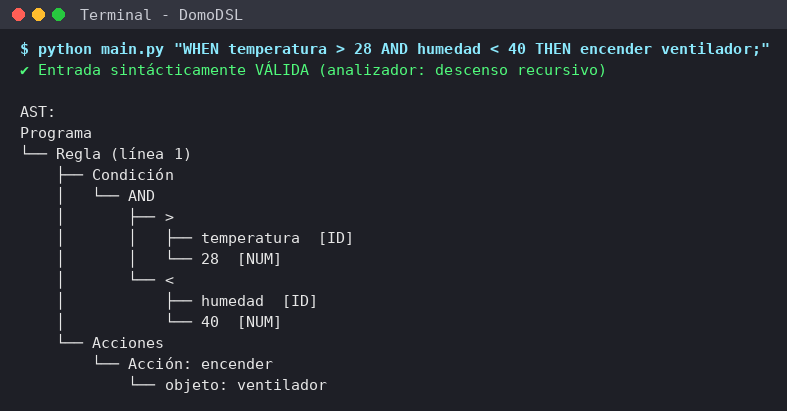
\includegraphics[width=0.78\textwidth]{../docs/img/cap_valida.png}
\caption{Entrada válida: se informa el resultado y se imprime el AST.}
\end{figure}
\begin{figure}[H]\centering
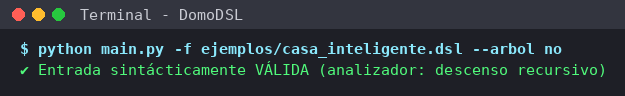
\includegraphics[width=0.95\textwidth]{../docs/img/cap_archivo.png}
\caption{Análisis de un archivo con cuatro reglas (\texttt{ejemplos/casa\_inteligente.dsl}).}
\end{figure}
\begin{figure}[H]\centering
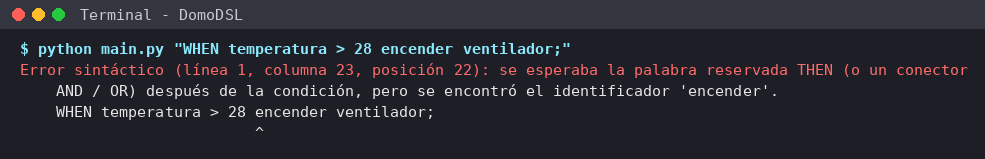
\includegraphics[width=0.95\textwidth]{../docs/img/cap_error_then.png}
\caption{Error sintáctico: falta \texttt{THEN}.}
\end{figure}
\begin{figure}[H]\centering
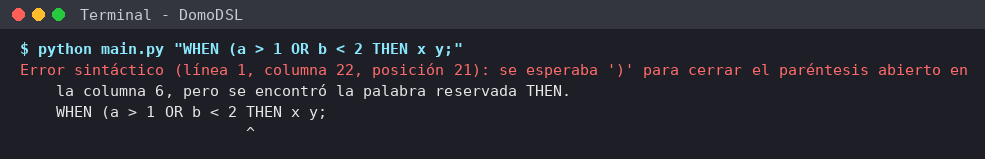
\includegraphics[width=0.95\textwidth]{../docs/img/cap_error_parentesis.png}
\caption{Error sintáctico: paréntesis sin cerrar.}
\end{figure}
\begin{figure}[H]\centering
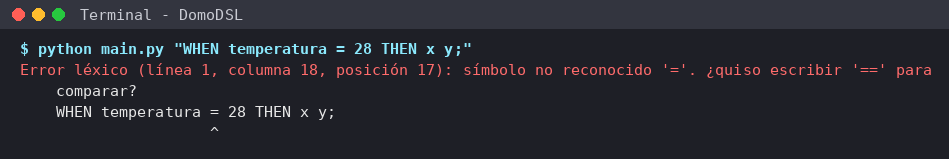
\includegraphics[width=0.95\textwidth]{../docs/img/cap_error_lexico.png}
\caption{Error léxico: \texttt{=} en lugar de \texttt{==}.}
\end{figure}
\begin{figure}[H]\centering
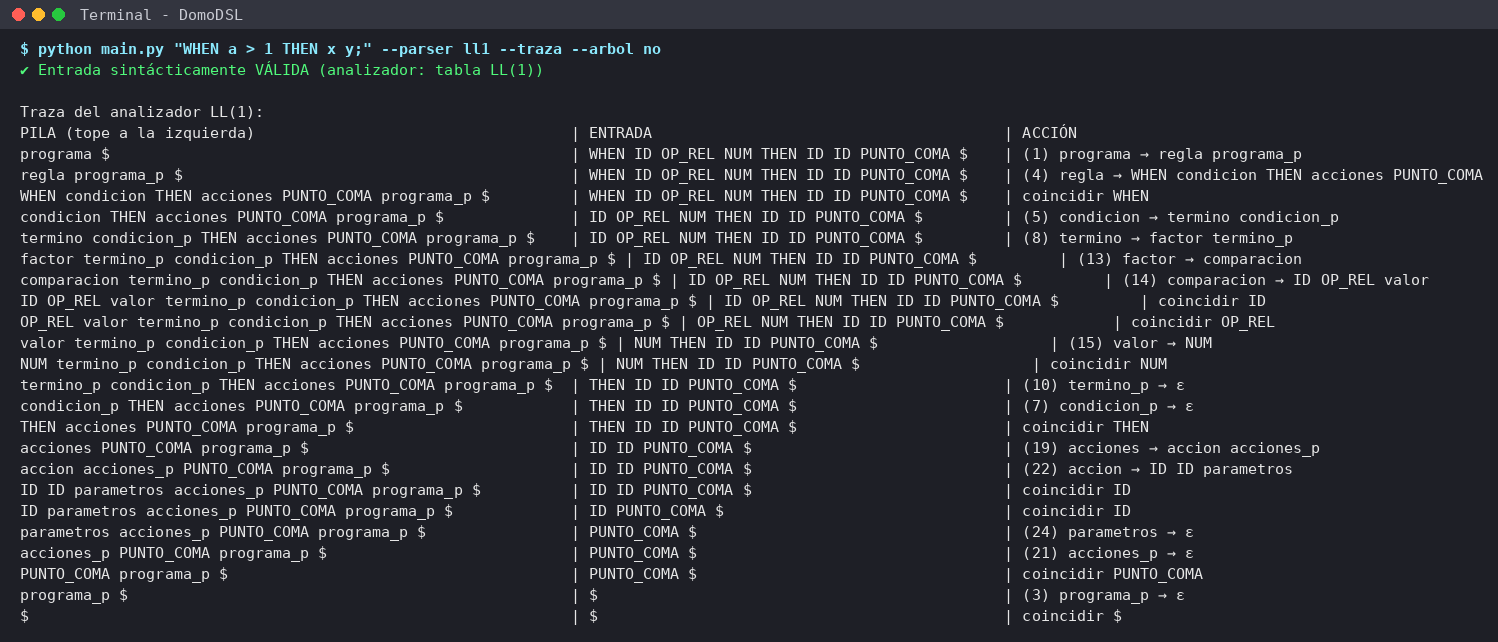
\includegraphics[width=\textwidth]{../docs/img/cap_traza_ll1.png}
\caption{Traza del analizador LL(1) (\texttt{--traza}): pila, entrada restante y producción aplicada.}
\end{figure}
\begin{figure}[H]\centering
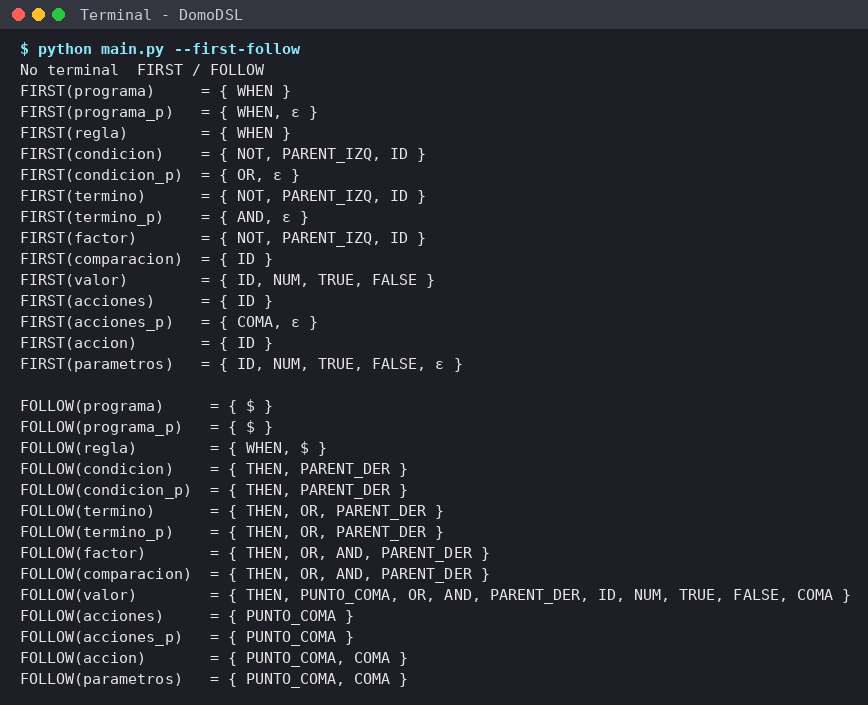
\includegraphics[width=0.85\textwidth]{../docs/img/cap_first_follow.png}
\caption{FIRST y FOLLOW calculados por el programa (\texttt{--first-follow}).}
\end{figure}
\begin{figure}[H]\centering
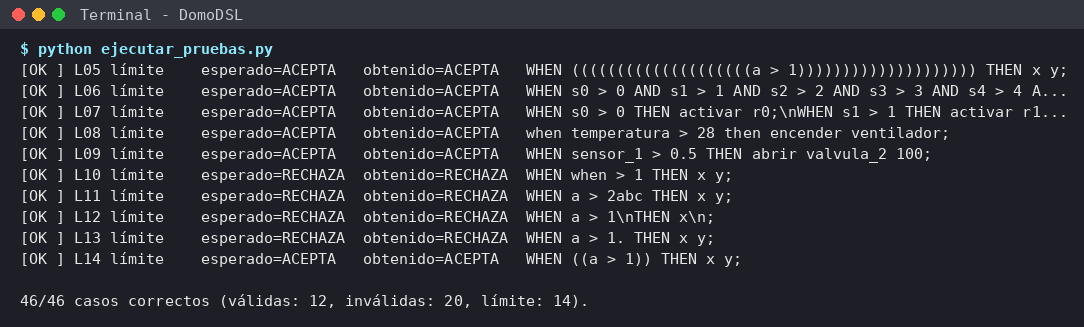
\includegraphics[width=0.95\textwidth]{../docs/img/cap_pruebas.png}
\caption{Resultado de \texttt{ejecutar\_pruebas.py}.}
\end{figure}
\begin{figure}[H]\centering
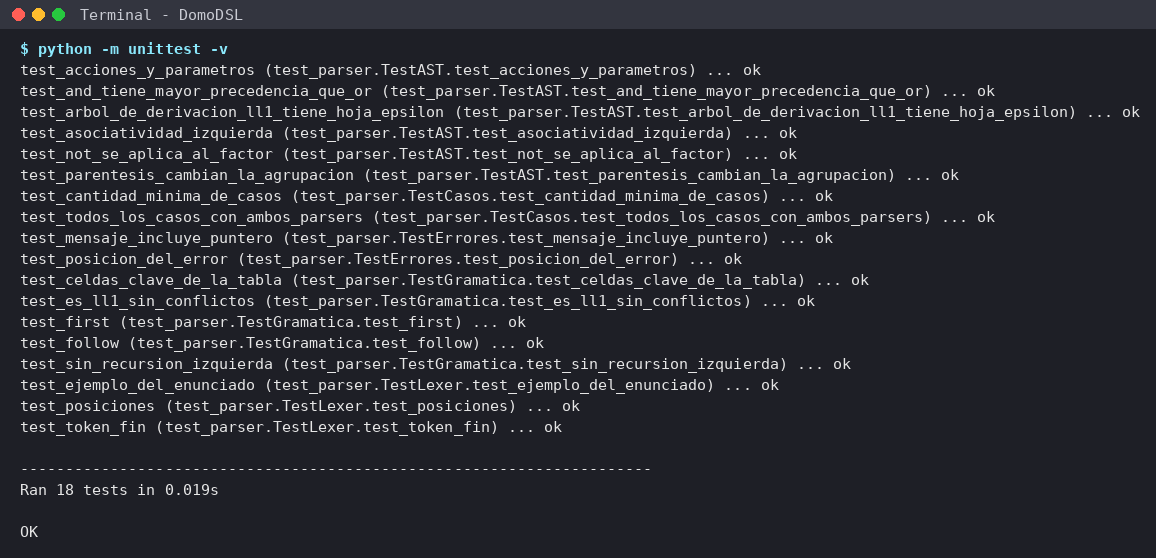
\includegraphics[width=0.95\textwidth]{../docs/img/cap_unittest.png}
\caption{Resultado de las pruebas unitarias.}
\end{figure}

\clearpage
\subsection*{Anexo C. Código fuente de los módulos principales}
\lstinputlisting[caption={lexer.py --- analizador léxico}]{../lexer.py}
\lstinputlisting[caption={gramatica.py --- GLC, FIRST, FOLLOW y tabla LL(1)}]{../gramatica.py}
\lstinputlisting[caption={parser\_rd.py --- parser por descenso recursivo}]{../parser_rd.py}
\lstinputlisting[caption={parser\_ll1.py --- parser dirigido por tabla LL(1)}]{../parser_ll1.py}

\fi
